%**************************************************************************************
% License:
% CC BY-NC-SA 4.0 (http://creativecommons.org/licenses/by-nc-sa/4.0/)
%**************************************************************************************

\documentclass[notes]{beamer}

\mode<presentation> {

\usetheme{Madrid}

% Burnt orange
\definecolor{burntorange}{rgb}{0.8, 0.33, 0.0}
\colorlet{beamer@blendedblue}{burntorange}
% Pale yellow
\definecolor{paleyellow}{rgb}{1.0, 1.0, 0.953}
\setbeamercolor{background canvas}{bg=paleyellow}
% Secondary and tertiary palett
\setbeamercolor*{palette secondary}{use=structure,fg=white,bg=burntorange!80!black}
\setbeamercolor*{palette tertiary}{use=structure,fg=white,bg=burntorange!60!black}

% To remove the footer line in all slides uncomment this line
%\setbeamertemplate{footline}
% To replace the footer line in all slides with a simple slide count uncomment this line
%\setbeamertemplate{footline}[page number]

% To remove the navigation symbols from the bottom of all slides uncomment this line
%\setbeamertemplate{navigation symbols}{}
}

\usepackage{amsmath}
\usepackage{bm}
\usepackage{breqn}
\usepackage{fontawesome}
\usepackage{graphicx} % for figures
\usepackage{subcaption} % for subplots 
\usepackage[labelsep=space,tableposition=top]{caption}
\renewcommand{\figurename}{Fig.} 
\usepackage{cleveref}
\usepackage{caption,subcaption}% http://ctan.org/pkg/{caption,subcaption}
\usepackage{booktabs} % Allows the use of \toprule, \midrule and \bottomrule in tables
\usepackage{multirow}
\usepackage{xcolor}
\usepackage{empheq}
\usepackage[most]{tcolorbox}
\usepackage{listings}% http://ctan.org/pkg/listings
\lstset{basicstyle=\ttfamily,breaklines=true}
\usepackage{siunitx}
\usepackage{verbatim}

% To print 2 slides on a page
%\usepackage{handoutWithNotes}
%\pgfpagesuselayout{2 on 1}[border shrink=2mm]
%----------------------------------------------------------------------------------------
%	TITLE PAGE
%----------------------------------------------------------------------------------------
% The short title appears at the bottom of every slide, the full title is only on the title page
\title[CE 311K: NR \& diff]{CE 311K: Newton Raphson and Differentiation} 
\author{Krishna Kumar} % name
\institute[UT Austin] % institution 
{
University of Texas at Austin \\
\medskip
\href{mailto:krishnak@utexas.edu}{krishnak@utexas.edu} % email address
}
\date{\today} % Date, can be changed to a custom date

\begin{document}

\begin{frame}
\titlepage % title page as the first slide
\end{frame}

\newif\ifshowtoc
\showtoctrue% toggles to show the toc

\AtBeginSection{%
	\ifshowtoc
	\begin{frame}
		\tableofcontents[currentsection, subsectionstyle=show/show/hide]
	\end{frame}
	\fi
}

\section{Newton Raphson}
%------------------------------------------------
\begin{frame}
	\frametitle{Newton Raphson}
 Assuming $r$ is a root of $f$ and that f is continuously differentiable in the
	vicinity of $r$ with $f^\prime (r) \ne 0$, then a sequence $(x_n)$ that converges to $r$ for $n \rightarrow \infty$ can be found using the Taylor expansion of $f$:
	\mode<beamer>{
		\begin{align*}
			f(r) & =  f(x_n + \varepsilon_n) = f(x_n) + f^\prime(x_n)\varepsilon_n + \frac{f^{\prime\prime}(x_n)}{2!}\varepsilon_n^2 \dots \\
			\varepsilon_n & \approx - \frac{f(x_n)}{f^\prime(x_n)} \\
			r = x_n + \varepsilon_n & \approx x_n - \frac{f(x_n)}{f^\prime(x_n)}
		\end{align*}
		in other words $ x_n - \frac{f(x_n)}{f^\prime(x_n)}$ is the next iteration of $r$, and hence we write:
	\begin{equation*}
	x_{n+1} = x_n - \frac{f(x_n)}{f^\prime(x_n)}
	\end{equation*} 
	}
	\mode<handout>{
		\vspace{5cm}
	}
\end{frame}
\note{
		We wish to find roots of $f(x)$ using a converging sequence $(x_n)$. But we want to do it faster.
		
	Newton's original method (1685) was purely algebraic, which he applied only to	polynomials and used a sequence of polynomials instead of successive approximations $x_n$.
	
	Raphson's simplified version (1690) was also only algebraic and he applied it only to polynomials but used $x_n$ approximations. 
	
	Simpson gave the form used today 50 years later (1740), along with other important results in the same paper.}


%------------------------------------------------
\begin{frame}
	\frametitle{Newton-Raphson graphical expression}
	\mode<beamer>{
		\begin{figure}[ht]
			\centering
			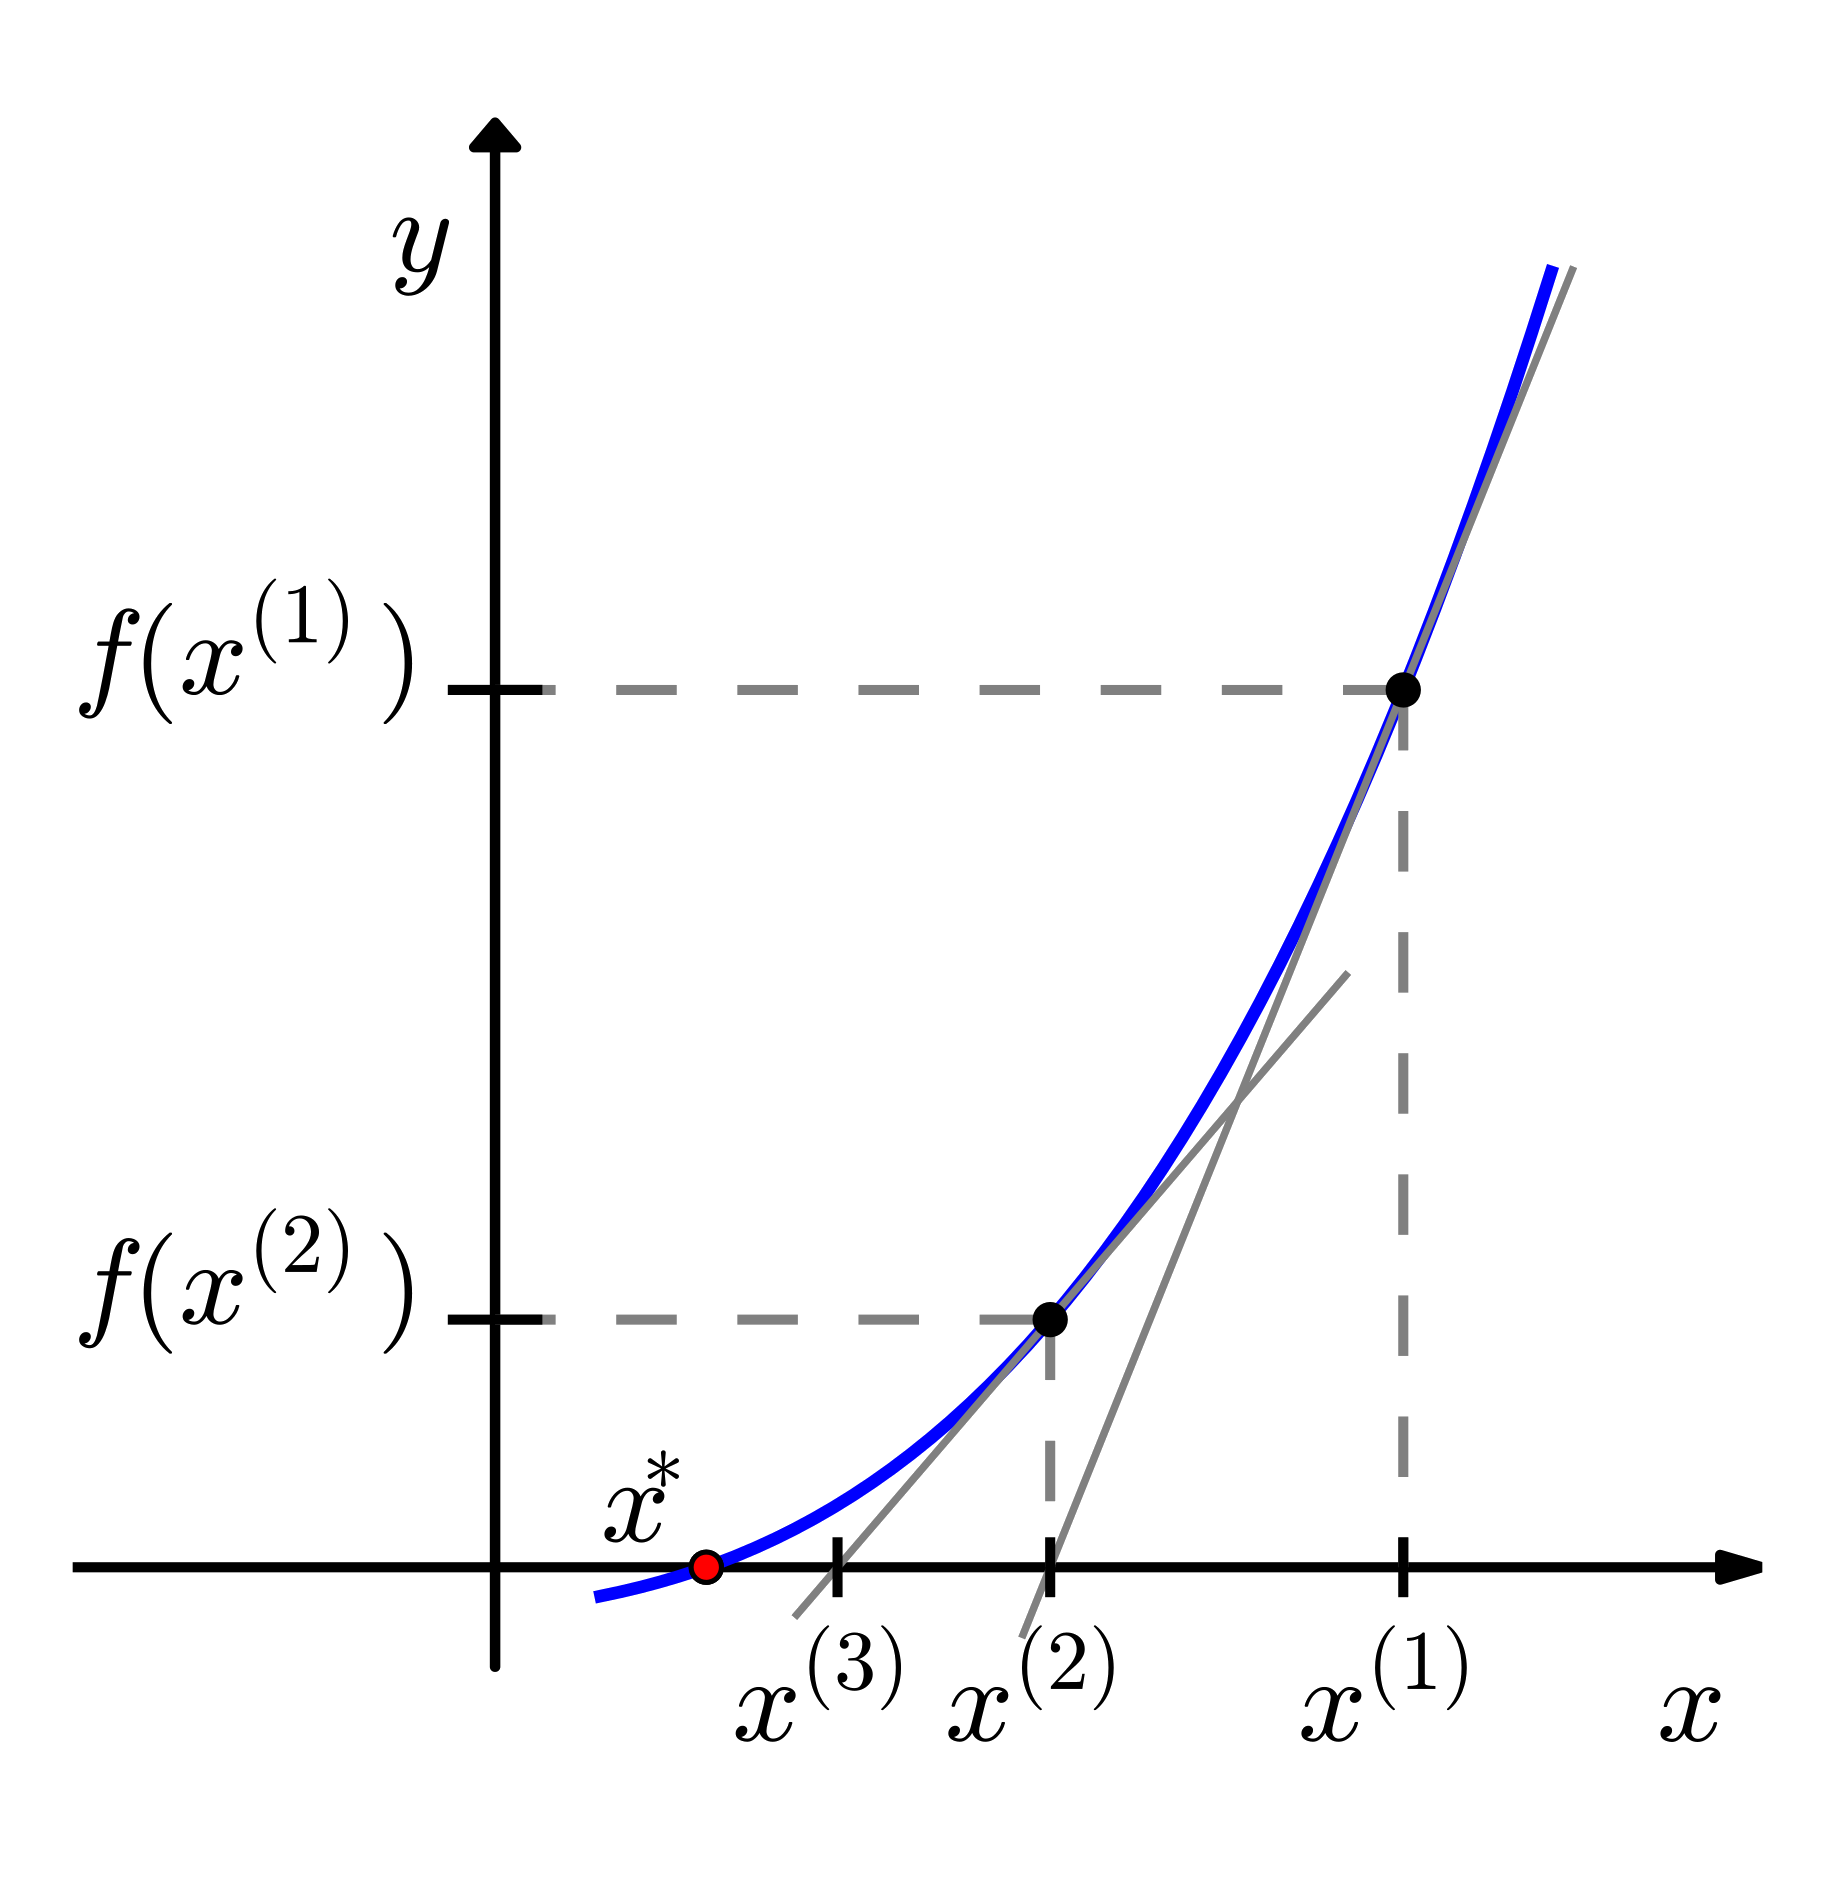
\includegraphics[width=0.65\textwidth]{figs/newton.png}
		\end{figure}
	}
	\mode<handout>{
		\vspace{5cm}
	}
\end{frame}

%------------------------------------------------
\begin{frame}
	\frametitle{Newton-Raphson failure}
	\begin{figure}[ht]
		\centering
		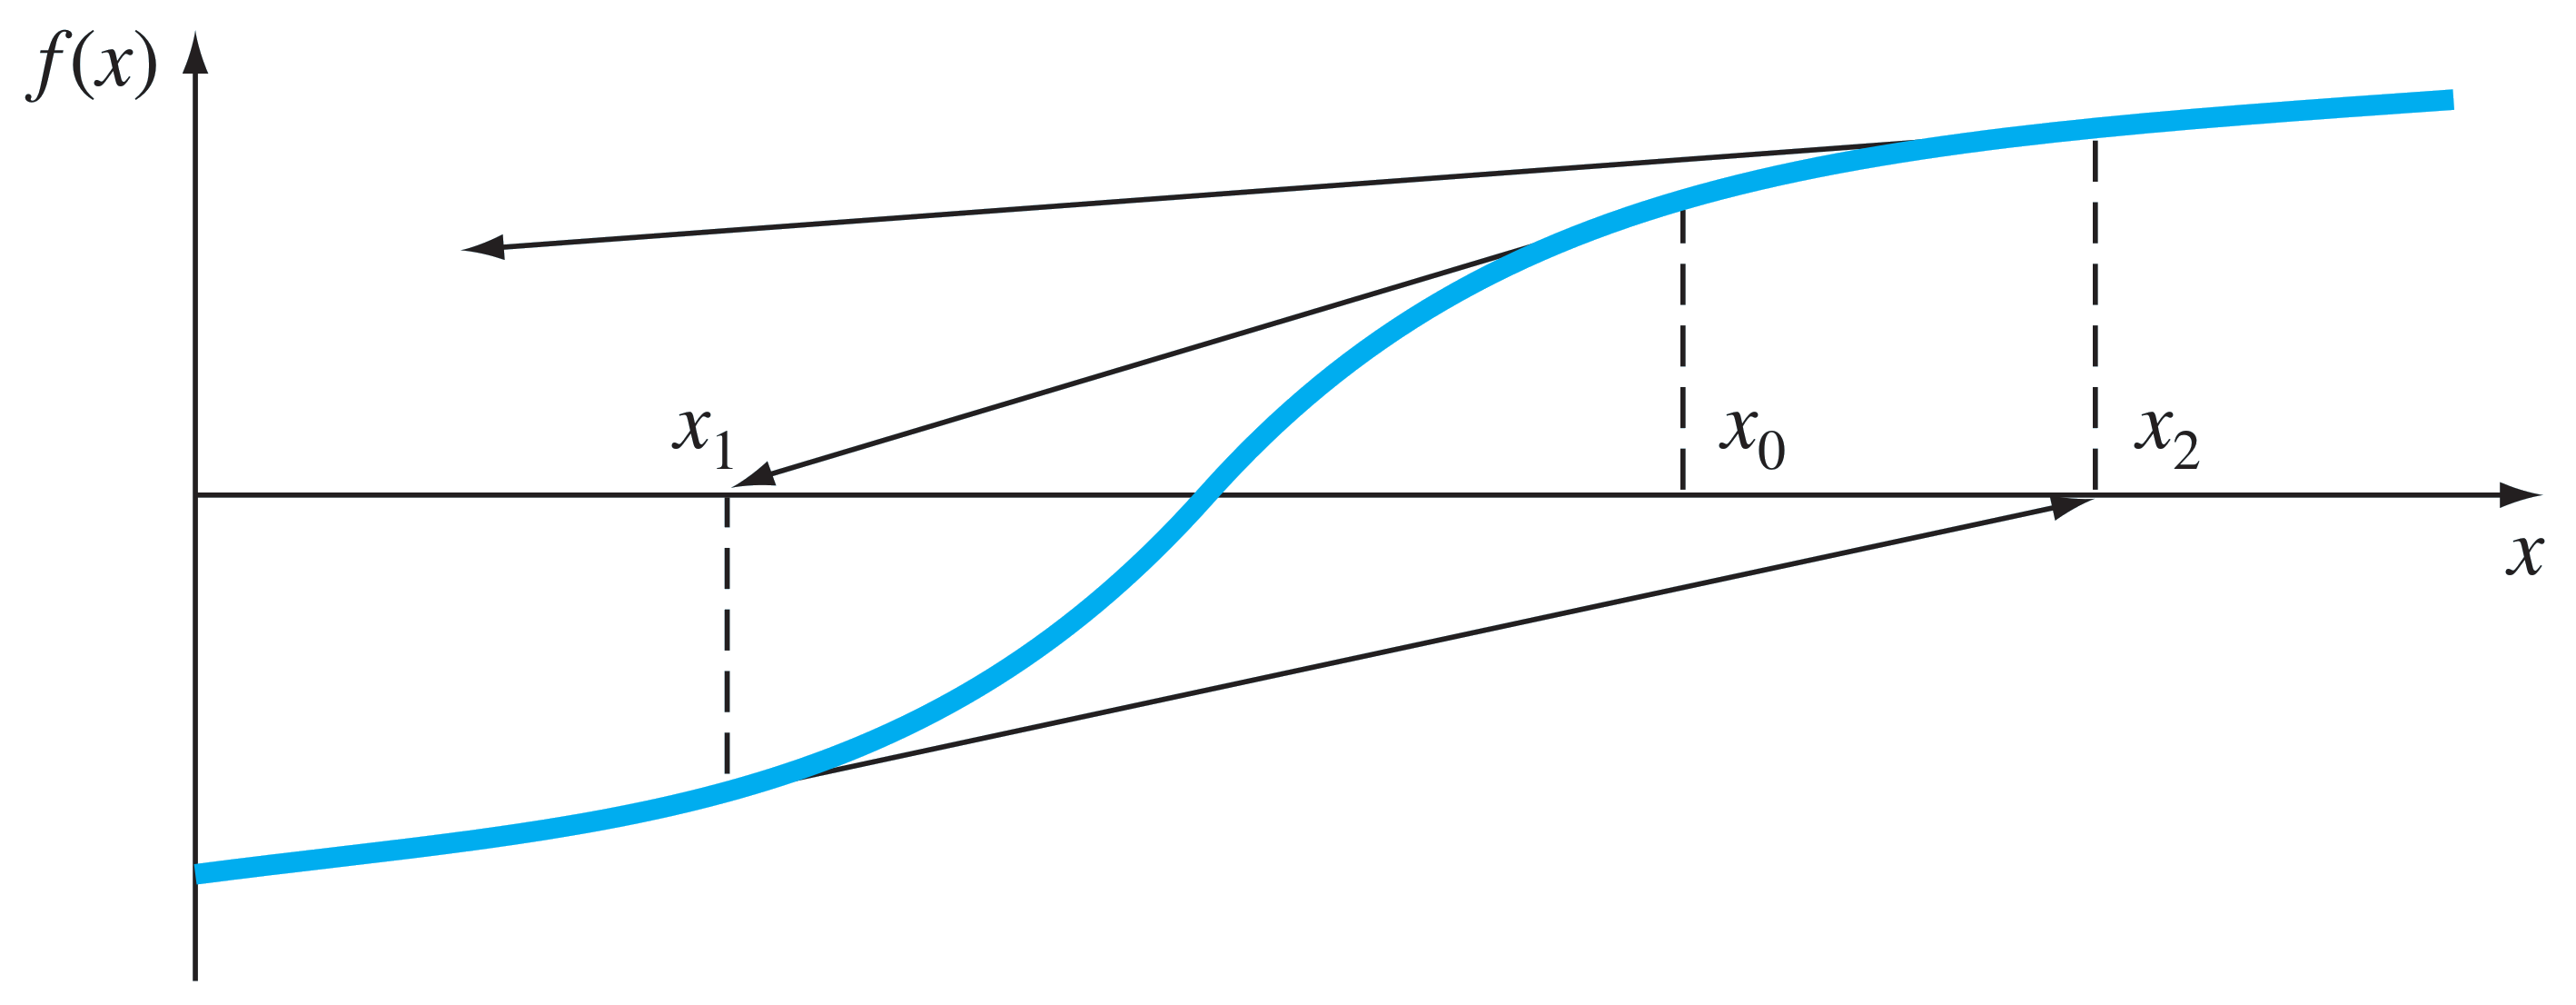
\includegraphics[width=\textwidth]{figs/nr-1.png}
	\end{figure}
\end{frame}


%------------------------------------------------
\begin{frame}
	\frametitle{Newton-Raphson failure}
	\begin{figure}[ht]
		\centering
		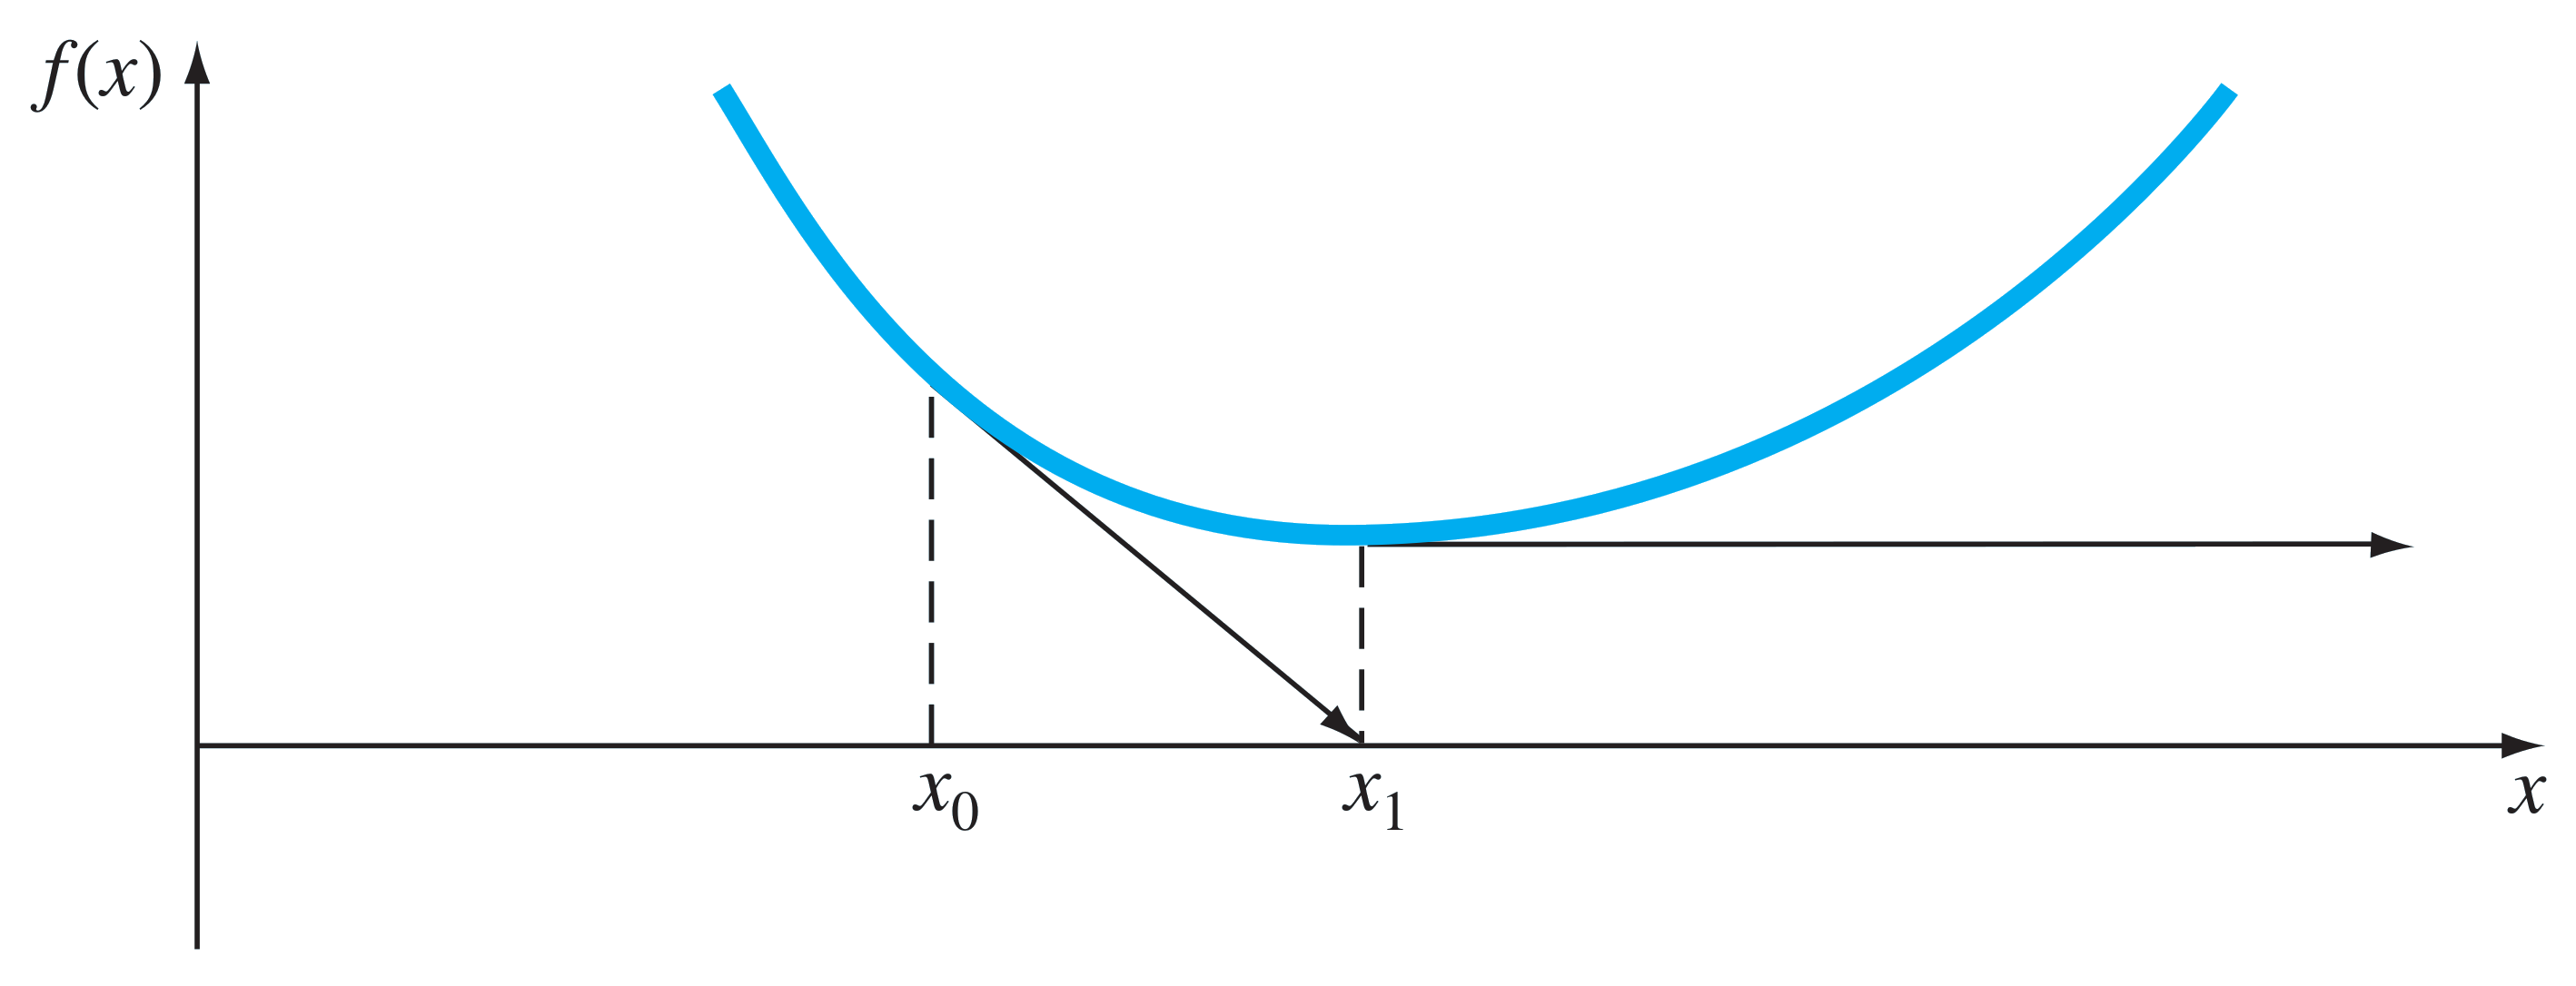
\includegraphics[width=\textwidth]{figs/nr-2.png}
	\end{figure}
\end{frame}

%------------------------------------------------
\begin{frame}
	\frametitle{Newton-Raphson failure}
	\begin{figure}[ht]
		\centering
		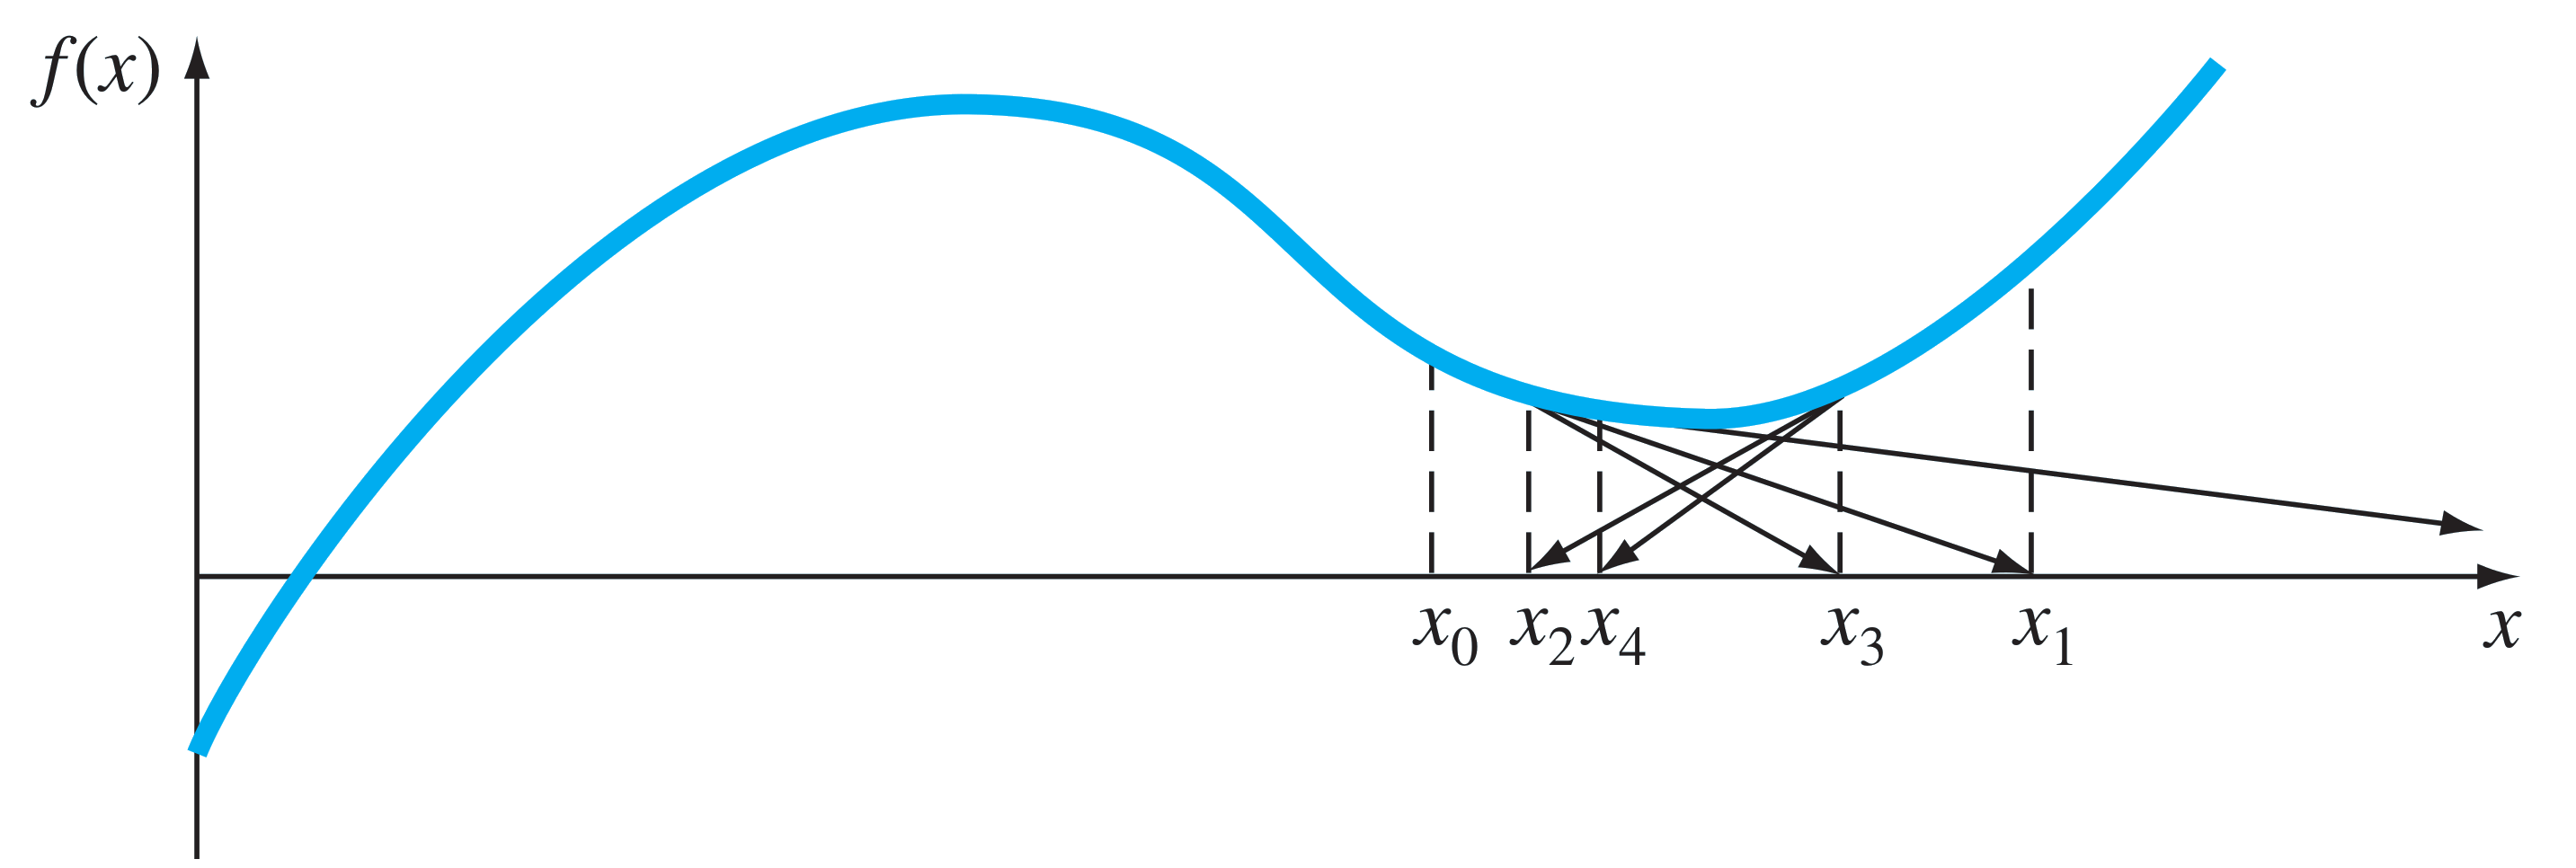
\includegraphics[width=\textwidth]{figs/nr-3.png}
	\end{figure}
\end{frame}

\end{document}
